\documentclass[12pt,a4paper]{ctexart}
\usepackage{titlesec,graphicx,amsmath,amssymb,tikz}
\usetikzlibrary{shapes.geometric,arrows}
\tikzstyle{startstop}=[rectangle,rounded corners,minimum width=1cm,minimum height=0.5cm,text centered,draw=black,fill=red!30]
\tikzstyle{process}=[rectangle,minimum width=1cm,minimum height=0.5cm,text centered,draw=black,fill=orange!30]
\tikzstyle{arrow}=[thick,->,>=stealth]
\graphicspath{{img/}}
\titleformat{\section}{\normalfont\large\bfseries}{\thesection}{1em}{}
\title{
    {\heiti\zihao{2} 大英四研究过程总结}\\
    {\songti\zihao{4} ————互联网抽象文化与网络暴力之间的关系}
}
\author{
    {\songti\zihao{4} 小组成员: 李维奇林, 潘翰霖, 张硕, 张书恺}\\
}
\date{最后更新: 2025.6.19}

\begin{document}
\maketitle
\tableofcontents
\newpage

\section{研究主要介绍}
\subsection{背景}

网络抽象文化源于网络主播为吸引观众而刻意采用的非常规行为与话术,其传播则是由反粉丝群体通过在微博等社交媒体平台发起系统性抹黑行动扩散直播冲突所推动。该文化呈现出三大典型特征:需特定知识解码的抽象化表达、特定社群内强烈的群体认同构建,以及通过夸张模仿解构主流规范的 pervasive irony(普遍反讽)\cite{zheng2024chinese}。

当这种抽象语言渗入主流网络文化时,其特质——尤其是对意义的反讽式解构——对数字传播产生了出人意料的影响。通过追踪特定词汇(如"牢大")在不同时期的语义演变,我们可以观察到抽象文化如何戏剧性地重塑词语的意义与内涵。这一过程有效解构了语义关联,剥离词汇原有的敌对意图,将其重塑为社会娱乐化的表达载体。

这种语言解构根植于挑战语言二元对立与等级结构的哲学传统\cite{liu2019deconstruction},在网络传播中呈现出鲜明特征。该过程呼应德里达对结构主义的批判——通过动摇固定意义,将传统携带对抗性价值判断的词汇(如优越/低劣、攻击性/中性)重新配置为中立或戏谑的能指。在网络暴力语境下,这种解构机制转化了原本具有攻击性的语汇:曾用于群体间攻击的术语通过集体再挪用逐渐消解其有害内涵。我们以"耄耋"为例进行量化研究,该词最初源于网络关于猫的论战(暗指"拜猫如父"的过度偶像化),后经抽象文化特有的反讽解构,最终成为宠物社群中无害甚至亲昵的表达。

\subsection{研究意义}

本研究试图揭示数字生态中抽象文化与网络暴力之间复杂的互动关系。

研究揭示了一种深刻的文化转型现象:当抽象语言渗入主流网络空间后,普通用户逐渐剥离了其原有的恶意意图。案例研究表明,这些表达通过广泛传播被重新诠释为中性的社会娱乐符号。这种集体再挪用机制——即用户从相同短语中衍生出不同且往往幽默的新含义——有效消解了词汇原本的攻击性内涵。

\subsection{研究的问题}

如何对语言的暴力性进行考察?

如何对交流中出现的抽象文化元素进行考察?

抽象文化对网络暴力有何影响?

\subsection{研究阶段性目标}

本研究旨在研究网络抽象文化文化与网络欺凌之间的复杂关系。研究综合考察互联网群体的认知和行为模式,研究如下展开:

基于抽象网络文化与网络霸凌的典型案例与特征,我们设计了一个分析框架,以考察抽象文化如何调节暴力表达。

我们利用包括视频平台的网络爬虫获取数据,通过基于自然语言处理(NLP)的评论分析在内的计算方法,我们追踪meme出现在不同视频内容背景中的语义与话题演变,同时评估对应评论区的网络霸凌现象水平,以量化meme的转变如何影响讨论空间中的攻击性水平。

通过对调查结果与行为数据进行分析,我们将展示抽象文化的流行对于充满攻击性的网络霸凌的影响。

\begin{figure}[htbp]
    \centering
    \resizebox{\textwidth}{!}{
        \begin{tikzpicture}[node distance=2cm]
            \node (start)[startstop]{抽象文化与网络暴力};
            \node (process1)[process,below of=start,yshift=0cm,xshift=-4cm]{抽象文化定义、性质等};
            \node (process2)[process,below of=start,yshift=0cm,xshift=4cm]{网络暴力定义、特征等};
            \node (process3)[process,below of=start,yshift=-2cm,xshift=0cm]{抽象文化与网络暴力关系};
            \node (process4)[process,below of=process3,yshift=0cm,xshift=0cm]{研究方法: 网络爬虫. (如NLP自然语言处理)};
            \node (process5)[process,below of=process4,yshift=0cm,xshift=-4.5cm]{追踪不同视频平台评论的抽象性变化};
            \node (process6)[process,below of=process4,yshift=0cm,xshift=4.5cm]{评估对应评论区的网络暴力水平};
            \node (process7)[process,below of=process4,yshift=-2cm,xshift=0cm]{数据分析. (例如网络语言抽象性和暴力性的相关性)};
            \node (end)[startstop,below of=process7,yshift=0cm,xshift=0cm]{分析和讨论研究结果: 抽象文化对网络暴力的影响};
            \draw [arrow] (start) -- (process1);
            \draw [arrow] (start) -- (process2);
            \draw [arrow] (process1) -- (process3);
            \draw [arrow] (process2) -- (process3);
            \draw [arrow] (process3) -- (process4);
            \draw [arrow] (process4) -- (process5);
            \draw [arrow] (process4) -- (process6);
            \draw [arrow] (process5) -- (process7);
            \draw [arrow] (process6) -- (process7);
            \draw [arrow] (process7) -- (end);
        \end{tikzpicture}
    }
    \caption{Research Framework}
    \label{fig:research_process}
\end{figure}
\newpage

\section{研究方法}

%\subsection{问卷调查}

\subsection{网络爬虫}

为探究抽象文化对网络语言特征的影响,我们设计并构建了基于词典与jieba分词工具的舆情评估系统,用以考察公众评论中对原生议题的关注度、评论攻击性及网络迷因传播度。该系统从话题相关性评估、攻击性评估和迷因关联评估三方面入手,通过构建多级词典与基于频次的量化方法,为评论区整体内容特征提供可视化与量化分析支持。

基于Python的视频评论区信息采集:自动化爬取bilibili指定视频评论及其多级回复。程序首先通过设置浏览器请求头模拟正常用户访问,避免被反爬机制拦截。主函数通过分页请求B站评论API,获取所有一级评论后,递归抓取每条评论下的二级及以下回复,确保评论数据完整性。每条评论及回复均提取用户昵称、评论内容、回复对象、评论层级、性别、评分、点赞数、回复时间等关键信息。所有获取的评论数据最终保存为CSV文件以供进一步分析。

\begin{figure}[htbp]
    \centering
    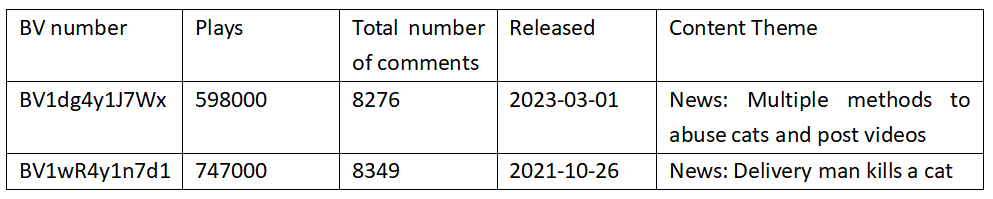
\includegraphics[width=0.8\textwidth]{img/data_sources_1.png}
    \caption{数据来源概览}
    \label{fig:data_sources_1}
\end{figure}
\newpage

对于用于词典构建的数据,我们采用了央视新闻与四川观察两则新闻报道的评论区,其较好地覆盖了"耄耋"梗衍生的"流浪猫问题"与"虐猫行为"议题,同时具备充足的评论数量,有利于准确获取词典内容。

\begin{figure}[htbp]
    \centering
    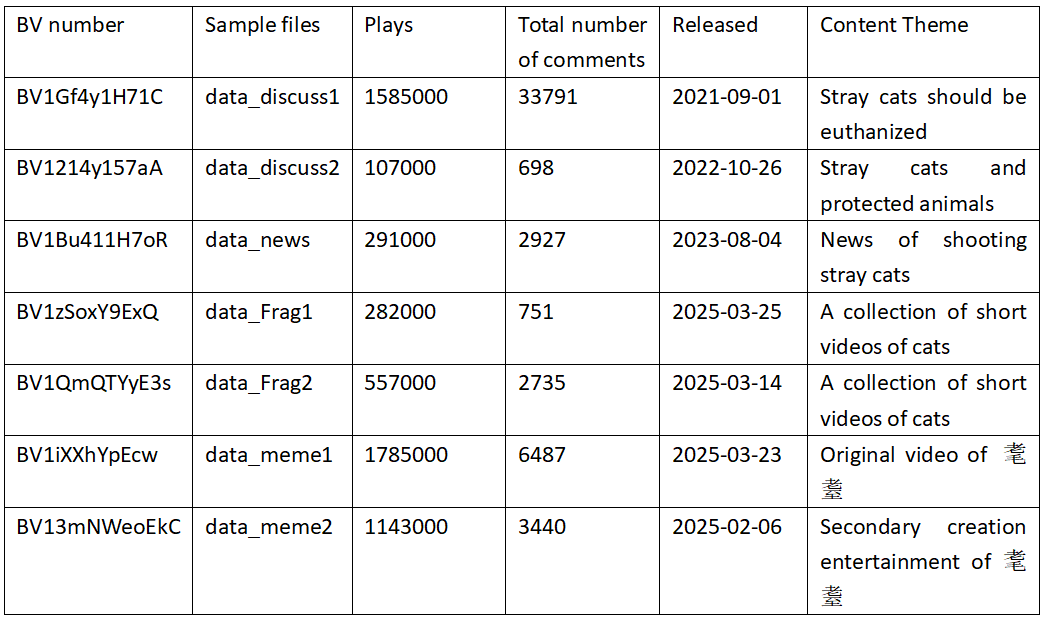
\includegraphics[width=0.8\textwidth]{img/data_sources_2.png}
    \caption{数据来源概览}
    \label{fig:data_sources_2}
\end{figure}
\newpage

根据人工筛查视频内容获得的多组不同主题视频样本,BV1Gf4y1H71C视频是探讨如何处理流浪猫问题的讨论,作者认为需通过安乐死解决流浪猫数量泛滥问题;BV1214y157aA作者使用激进语言表达对流浪猫作为入侵物种威胁生态的批判;BV1Bu411H7oR是某小区居民用弓箭射杀流浪猫的新闻报道;BV1zSoxY9ExQ与BV1QmQTYyE3s为猫咪行为短视频合集;BV1iXXhYpEcw记录了一只流浪猫闯入民宅并展现极端攻击性的过程,该事件现被抽象文化广泛称为"耄耋"事件。BV13mNWeoEkC则是利用"耄耋"事件视频素材创作的鬼畜娱乐视频。

由于三个评估体系的内容均为自然语言文本,直观的评估方式即对特定文本内容进行统计评估。因此研究首先需要建立词典。

为全面客观界定"耄耋"梗发生场景与流浪猫问题讨论的主要方向与主题,本研究首先采集了两则流浪猫问题新闻视频的评论区数据,通过统计评论区高频词并人工筛查流浪猫问题讨论细节,获得能全面反映流浪猫问题讨论细节的话题相关性词典内容。

jieba:一款高效易用的中文分词工具,能准确将连续中文文本切分为词语,支持精确模式、全模式和搜索引擎模式三种分词模式,并允许用户通过自定义词典优化特定领域的分词效果。同时提供关键词提取与词性标注功能,广泛应用于文本分析、信息检索与自然语言处理任务,是处理中文文本的基础工具之一。

结合jieba的语言情感色彩分析,我们对上述高频词进行二次筛选,获得负面情绪较明显的高频词,这些词汇显然不仅具有较强的攻击性,同时与流浪猫讨论具有更强的相关性,从而获得更精确的评论区攻击性词典内容判断。

LDA:一种经典的无监督机器学习算法,主要用于文本数据的主题建模。它通过分析文档中词语的分布情况,自动识别潜在的文本主题结构,并将每个文档表示为多个主题的概率混合,同时每个主题表示为一组相关词语的概率分布。

基于预设词典的迷因关联评估:程序自动识别每个文件中的"评论内容"与"点赞"字段,判断每条评论是否包含指定的一级或二级迷因关键词。若一级关键词出现在评论中,则根据点赞数进行分值累加(点赞数为0则计1分),出现二级关键词则分值加1。任何包含提示关键词的评论均计入"提示评论"。最终程序统计每个文件的有效评论总数、迷因评论数及标准化迷因影响力分数(总分/评论数),并以柱状图形式展示各文件的迷因影响力,同时在终端输出详细统计结果,便于详细比较迷因在不同数据源中的传播与影响情况。

基于预设词典的话题相关性评估:程序实现对多个CSV评论数据文件中"迷因"原生语境偏移的分析。程序自动识别每个文件中评论的内容,对每条评论进行分词,并根据自定义分级词典(一级、二级、三级)为每个词语分配不同分值(4分、2分和1分)。在累计每条评论的得分后,计算每个文件的平均原生指数,并以条形图形式展示各文件的原生指数分布。程序还将在终端输出每个文件的评论总数与平均原生指数,便于直观比较分析不同数据源中"迷因"语境的原生性与偏移程度。

为考察评论区讨论内容的特征,我们结合jieba与LDA实现了中文文本主题分析系统:通过LDA主题建模提取每个文档评论内容的核心主题及关键词分布。系统首先对原始文本进行中文分词、停用词过滤等预处理,随后构建词频矩阵并训练LDA模型,识别每个文件中五个主要主题及其代表关键词。通过计算归一化熵值量化主题多样性,最终生成可视化结果。

结合jieba与词典的攻击性评估:程序自动识别每个文件中评论内容与点赞数,对每条评论进行分词,并根据自定义攻击性词典对攻击性词语赋予不同权重,基于点赞数加权累计计算每个文件的总攻击性分数。最终程序对评论攻击性指数进行归一化处理,以柱状图形式展示各文件的攻击性等级,并在终端输出每个文件的评论总数与攻击性指数,便于直观比较分析不同数据源中攻击性评论的分布与强度。

\section{研究结果}%数据呈现与结果分析

%\subsection{问卷调查结果呈现}

\subsection{网络爬虫结果呈现}

首先通过抽象性评估对七个评论区数据进行评测,统计结果显示可以观测到模因在七个评论区的出现情况,展现出良好相关性。这为数据选择的合理性提供了支撑。

\begin{tabular}{|l|c|c|}
    \hline
    数据文件 & 原始分数 & 评论总数 \
    \hline
    data discuss1 & 6783 & 11608 \
    data discuss2 & 118 & 304 \
    data news & 442 & 1458 \
    data Frag1 & 165 & 480 \
    data Frag2 & 788 & 1667 \
    data meme1 & 795 & 3205 \
    data meme2 & 78 & 2369 \
    \hline
\end{tabular}

\begin{figure}[htbp]
    \centering
    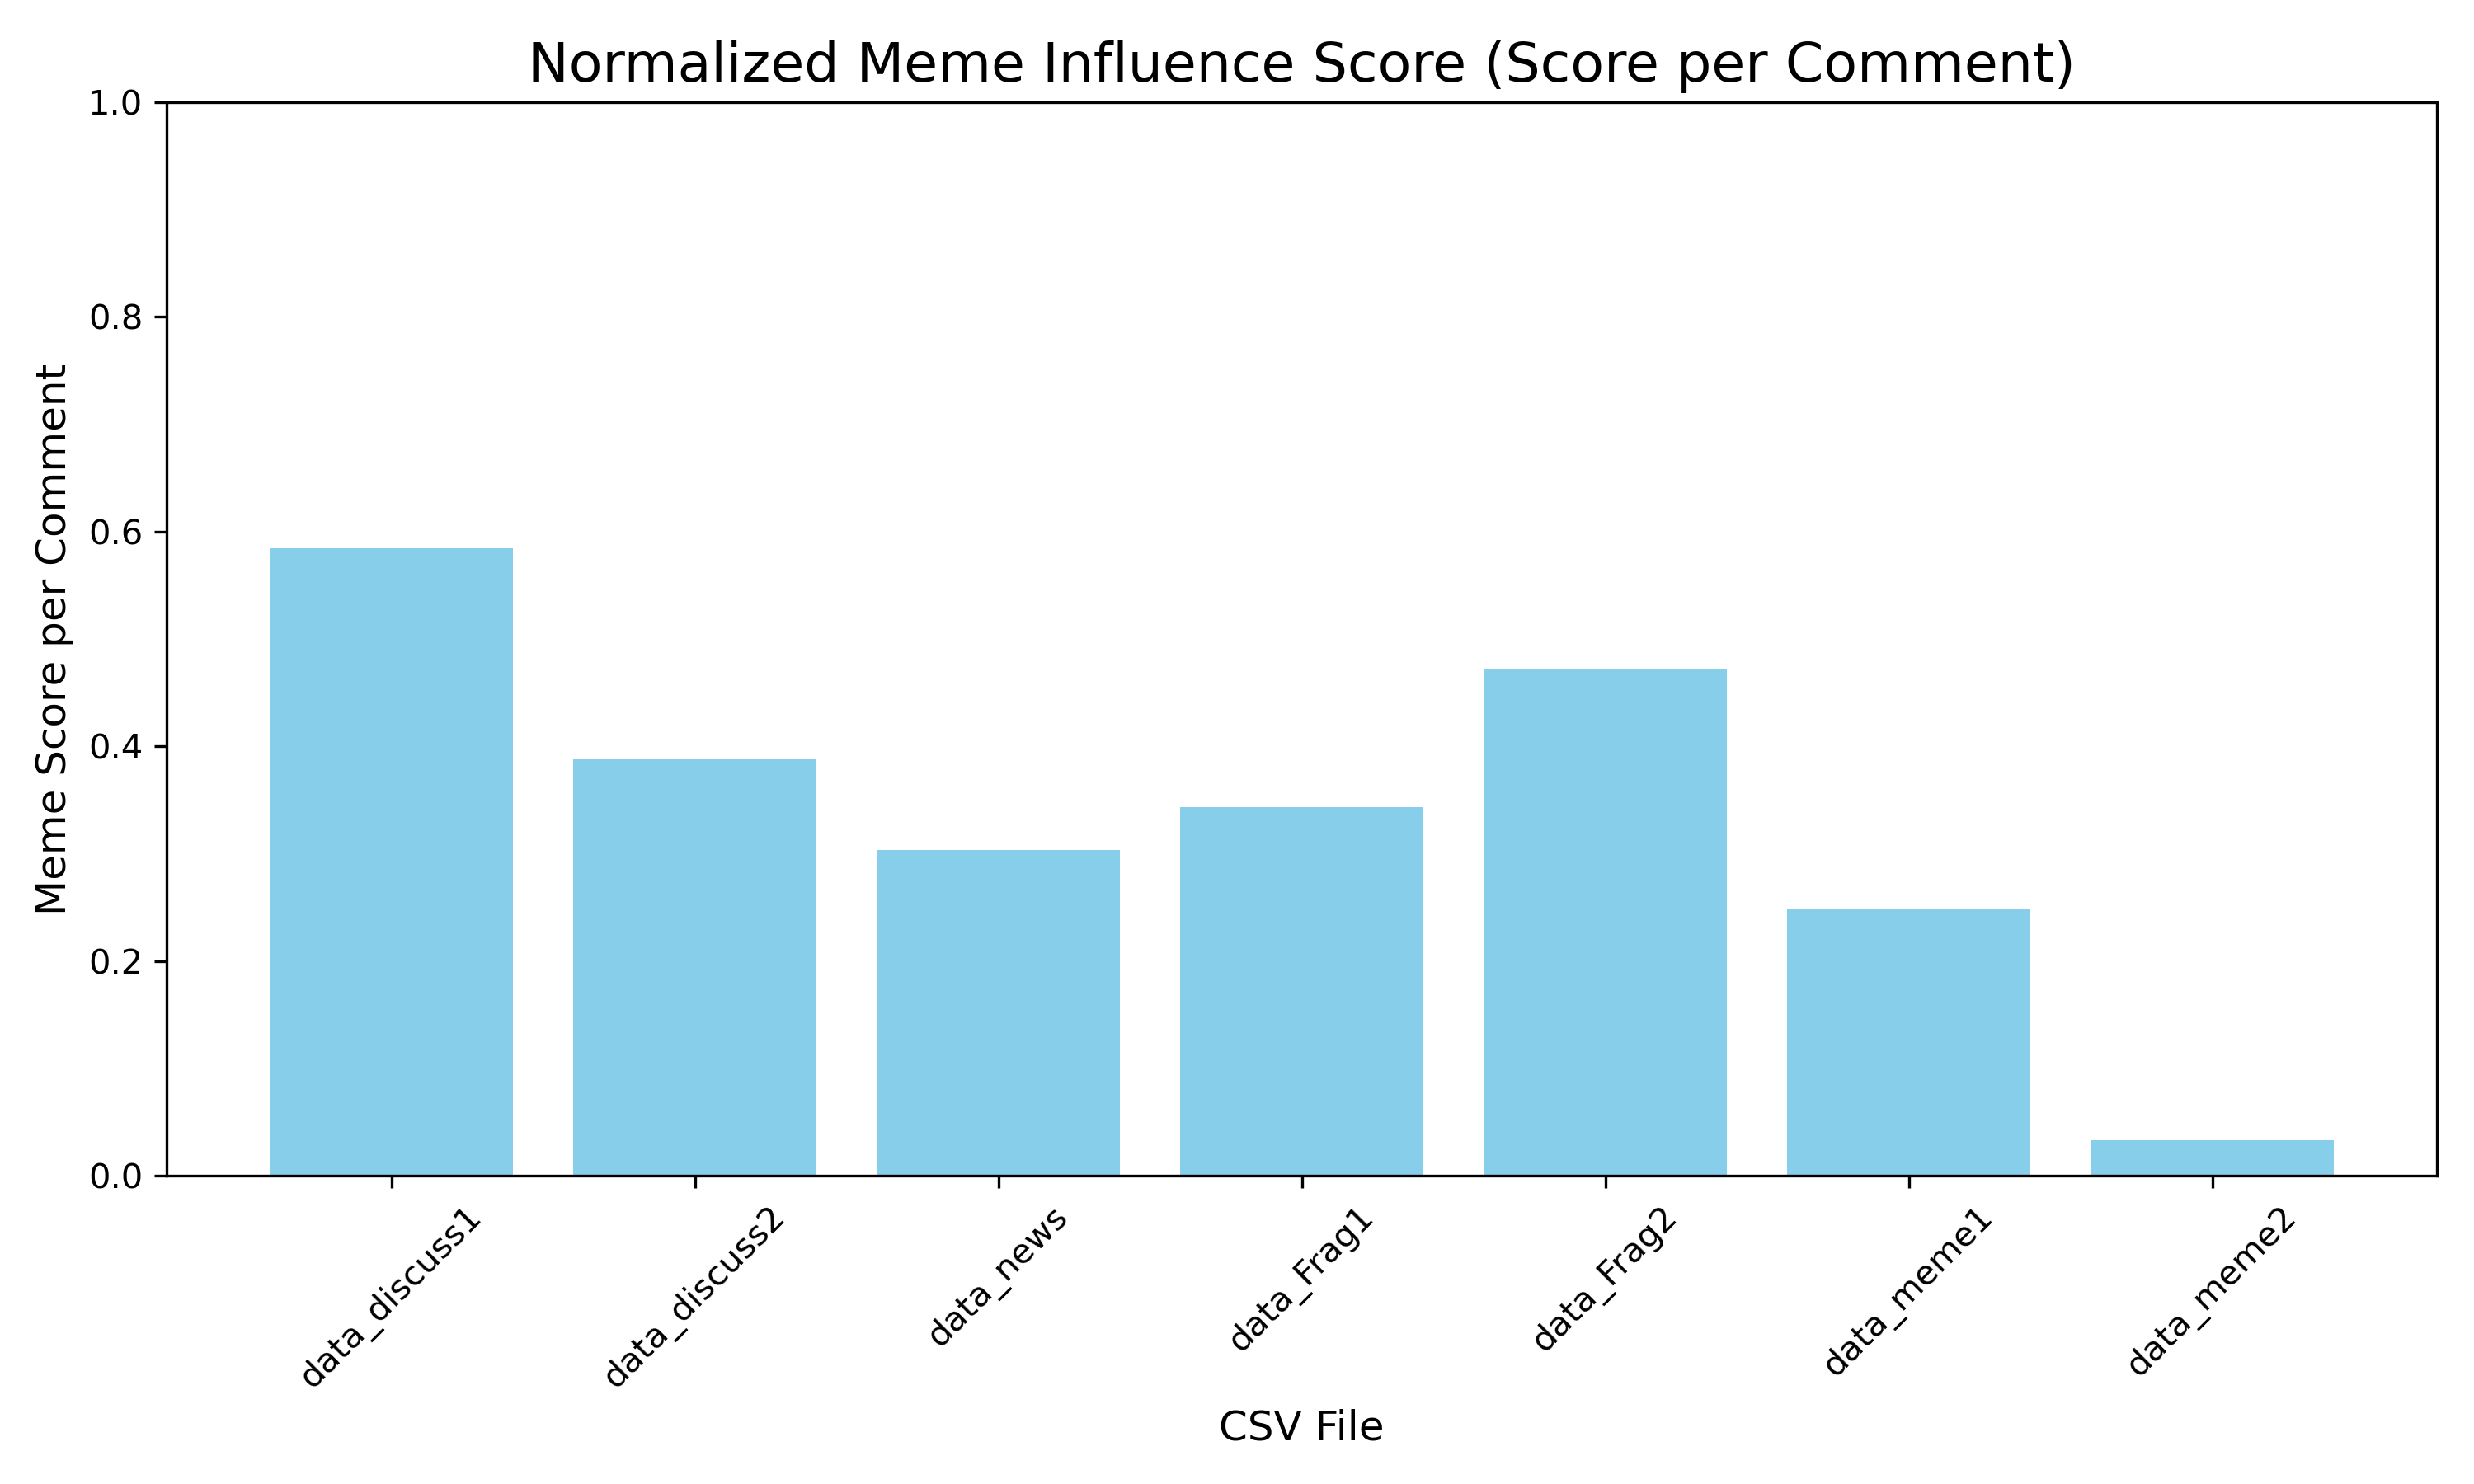
\includegraphics[width=0.8\textwidth]{img/meme_score.png}
    \caption{抽象性评分分布}
\end{figure}
\newpage

随后通过攻击性评估对七个评论区数据进行评测,统计结果如下:可见直接讨论流浪猫问题的两个视频和关于流浪猫新闻的视频评论区表现出明显更强的攻击性,而基于流浪猫问题二次创作的两个视频语言攻击性显著低于其他样本。

\begin{figure}[htbp]
    \centering
    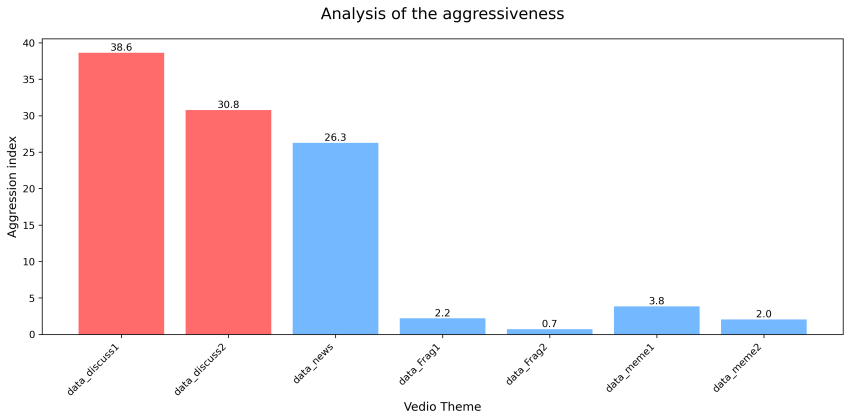
\includegraphics[width=0.8\textwidth]{img/aggressive_analysis.png}
    \caption{攻击性评估对比}
\end{figure}
\newpage

基于攻击性评估,对评论区言论攻击性进行评价,并根据发布时间统计同日评论攻击性平均水平,得到评论区攻击性随时间分布情况。

统计结果如下:

\begin{itemize}
    \item data discuss1.csv | 评论量:11608 | 2021-09-01 ~ 2025-05-14
    \item data discuss2.csv | 评论量:304 | 2022-10-26 ~ 2024-02-22
    \item data news.csv | 评论量:1458 | 2023-08-04 ~ 2025-05-14
    \item data Frag1.csv | 评论量:480 | 2025-03-25 ~ 2025-05-14
    \item data Frag2.csv | 评论量:1667 | 2025-03-19 ~ 2025-05-13
    \item data meme1.csv | 评论量:3205 | 2025-03-23 ~ 2025-05-14
    \item data meme2.csv | 评论量:2369 | 2025-02-06 ~ 2025-05-14
\end{itemize}

\begin{figure}[htbp]
    \centering
    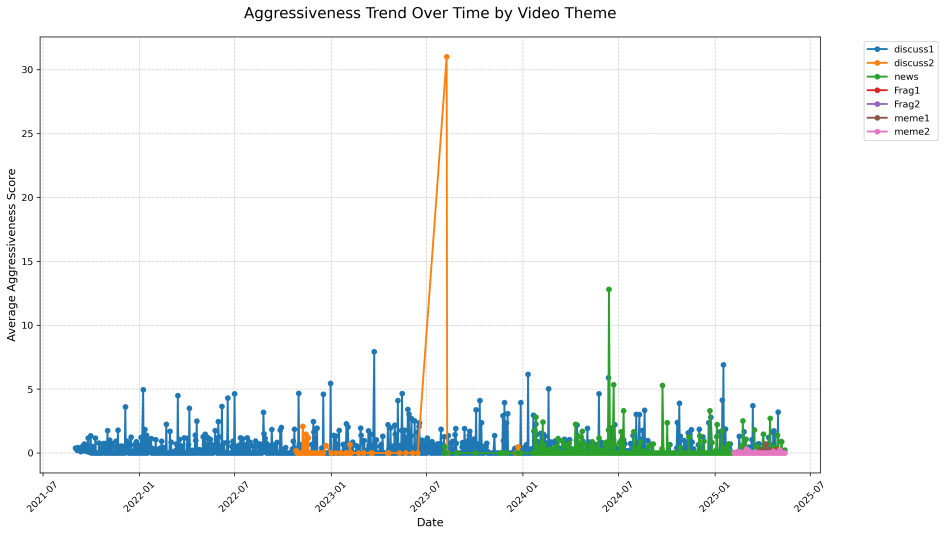
\includegraphics[width=0.8\textwidth]{img/aggressive_trend.png}
    \caption{攻击性趋势演变}
\end{figure}
\newpage

关于流浪猫的讨论视频评论区呈现出显著的高攻击性水平,表现为两种不同形态:一种长期保持明显较高的攻击性水平,另一种则出现远高于其他评论区攻击性水平的峰值。

流浪猫相关新闻视频评论区攻击性较强,但这种攻击性在达到峰值后逐渐减弱。

其他作品的评论区攻击性明显较低,且大多不存在较大波动。

可见从样本"discuss1"到"meme2"的评论区话题相关性呈现下降趋势,这意味着随着视频主题的偏移,评论区对流浪猫议题的讨论明显减少,且随着"耄耋"迷因的流行,该词汇已不再仅用于讨论流浪猫时使用。

\begin{figure}[htbp]
    \centering
    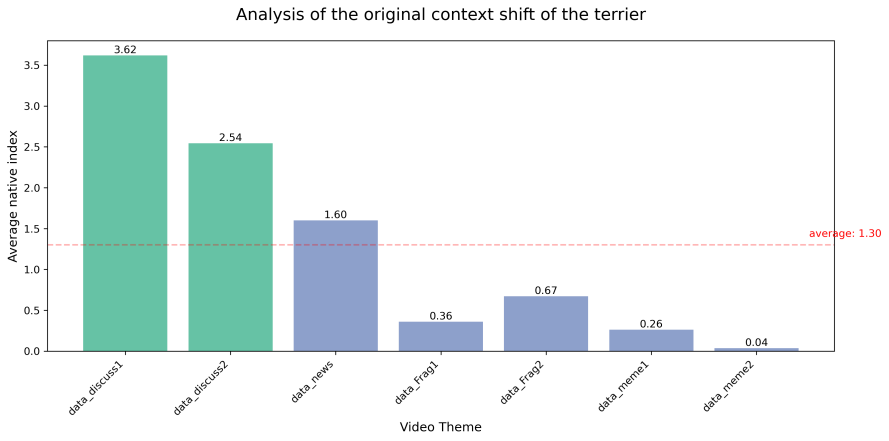
\includegraphics[width=0.8\textwidth]{img/context_shift.png}
    \caption{语境偏移趋势}
\end{figure}
\newpage

结合主题多样性评估系统,我们提取了七个评论区讨论的热门话题,统计结果如下:

\begin{itemize}
    \item \textbf{data discuss1}:
    \begin{itemize}
        \item Topic 1: 流浪, 一只, 喜欢, 真的, 绝育, 小区, 但是, 领养, 知道, 就是
        \item Topic 2: 流浪, 安乐死, 问题, 绝育, 捕杀, 人士, 就是, 不是, 爱猫, 直接
        \item Topic 3: 回复, 视频, doge, up, 这个, 老鼠, 评论, 一个, 建议, 一下
        \item Topic 4: 生态, 家猫, 我国, 人类, 老鼠, 就是, 这个, 还是, 论文, 物种
        \item Topic 5: 流浪, 人类, 动物, 物种, 城市, 数量, 生态, 因为, 不是, 就是
    \end{itemize}
    \item \textbf{data discuss2}:
    \begin{itemize}
        \item Topic 1: 流浪, 哈哈哈哈, 哈哈哈, 喜欢, 微笑, 可爱, 觉得, 真的, call, 不是
        \item Topic 2: doge, 脱单, 流浪, 回复, 吃瓜, up, 人类, 清道夫, 喜欢, 视频
        \item Topic 3: up, 滑稽, 建议, 小黑子, 不想, 流浪, 关注, 蟑螂, 是不是, 扑杀
        \item Topic 4: 物种, 流浪, 入侵, 危害, 放生, doge, 本土, 这么, 处理, 不能
        \item Topic 5: 流浪, 动物, 保护, 一个, 还是, 如果, 喜欢, 不是, 应该, 领养
    \end{itemize}
    \item \textbf{data news}:
    \begin{itemize}
        \item Topic 1: 垃圾, 这个, 射箭, 视频, up, 精英, 合肥, 不是, 如果, 邀请赛
        \item Topic 2: 流浪, 动物, 物种, 捕杀, 保护, 亿只, 造成, 生态, 入侵, 鸟类
        \item Topic 3: 流浪, 还是, 哈基米, 小区, 弓箭, 这种, 别人, 不是, 容易, 东西
        \item Topic 4: 回复, 就是, 野猫, 真的, 哔哩, 流浪, 一下, 人类, 喜欢, 要是
        \item Topic 5: 致敬, 传奇, 英雄, 支持, 复合弓, 韦鲁斯, 危险, 建议, 处理, 弹弓
    \end{itemize}
    \item \textbf{data Frag1}:
    \begin{itemize}
        \item Topic 1: 眼睛, 老鼠, 暹罗, tv, 哈吉, 还是, 真的, 这个, 支持, 音乐
        \item Topic 2: 我家, 星星, 这个, 知道, 一只, 豪猫, 神人, 就是, 忍住, 还是
        \item Topic 3: 喜欢, 养猫, 这么, 这种, 不如, doge, 穿越, 看片, 东西, 起来
        \item Topic 4: doge, 金箍, 主人, 一个, 突然, 回复, 耗子, 猫猫, 永远, 攻击
        \item Topic 5: 哈气, 养猫, 应激, 视频, 家里, 这些, 笼子, 直接, 足球, 你们
    \end{itemize}
    \item \textbf{data Frag2}:
    \begin{itemize}
        \item Topic 1: doge, 智商, 刺猬, 看到, 鼠饼, 一次, 狗饼, 出来, 还有, 见过
        \item Topic 2: 看到, 就是, 直接, 过去, 马路, 知道, 体型, 经常, 比较, 所以
        \item Topic 3: 原因, 滑稽, 就是, 撞死, 红绿灯, 我家, 小猫, 见到, 比较, 缝缝补补
        \item Topic 4: 因为, 聪明, 还是, doge, 流浪狗, 一般, 主要, 不是, 而且, 金箍
        \item Topic 5: 看见, 哈气, 哈基米, 狗子, 看到, 高速, 时候, 一个, 不少, 压死
    \end{itemize}
    \item \textbf{data meme1}:
    \begin{itemize}
        \item Topic 1: 不是, 野猫, 一只, 流浪, 经典, 还是, 但是, 这种, 如果, 这么
        \item Topic 2: 啊啊啊, 足球, 表情, 星星, 一个, 已经, 我力, 骇死, 宝宝, 汤圆
        \item Topic 3: doge, 这个, 这种, 金箍, 视频, 哈基人, 手套, 飞舞, 遇到, 那个
        \item Topic 4: 直接, 哈基米, 我家, 这样, 哈基, 然后, 基米, 神人, 过去, 忍住
        \item Topic 5: 哈气, 可爱, 知道, 相思, 就是, 哈基米, 圆头, 大哭, 感觉, 这猫
    \end{itemize}
    \item \textbf{data meme2}:
    \begin{itemize}
        \item Topic 1: 原版, 猎奇, 这个, 感觉, 武器, 眼睛, 吓人, 可爱, 哈基米, 超越
        \item Topic 2: 骇死, 我力, doge, 补档, 啊呀, 缓存, 视频, 还有, 这么, byd
        \item Topic 3: 视频, 出来, 恐怖, 真的, 一个, 支持, 这个, 孩子, 东西, 一只
        \item Topic 4: 哈气, 回复, 表情, 这个, mygo, 哔哩, 视频, 不是, 因为, 喜欢
        \item Topic 5: 看过, 微笑, official, 还原, 知道, tv, 程度, 不要, 一下, 骇人
    \end{itemize}
\end{itemize}

\begin{figure}[htbp]
    \centering
    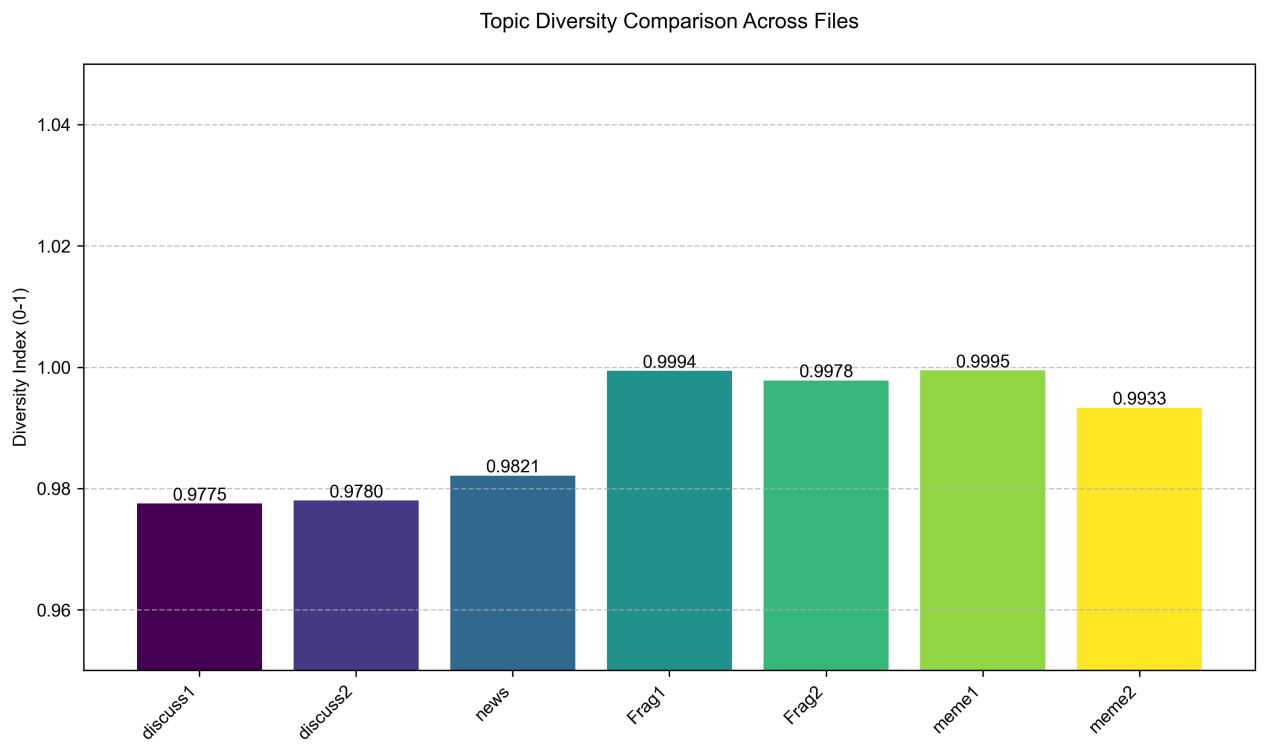
\includegraphics[width=0.8\textwidth]{img/topic_diversity.png}
    \caption{主题多样性分析}
\end{figure}
\newpage

研究发现:关于猫的主题讨论逐渐减少,评论区出现更多"哈基米"、"骇入"等抽象文化,且在攻击性评估得分较高的流浪猫讨论视频中,主题多样性明显较低。

\subsection{网络爬虫结果分析}

随着抽象文化的流行,其语境逐渐脱离原生议题,演变为独立的网络文化现象。

评论区攻击性与话题性质高度相关,严肃社会议题易引发高攻击性讨论,而随着抽象文化的流行,话题转向更具娱乐性的非严肃主题,这对语言暴力呈现出消解作用。

主题分析揭示了网络语言从实际问题讨论向多元抽象文化发展的趋势。

本实验为理解抽象文化对网络语言特征的影响提供了量化依据,揭示了攻击性语言在网络讨论中的动态变化特征。

\section{Discussion}

本实验通过对网络空间中网民的各种情况的调查,特别是对视频网站的评论语言的分析,对抽象文化和网络暴力的关系进行了初步的探索。
%删去对问卷结果的讨论
%抽象文化的流行性在年轻人中具有普遍性,问卷调查的参与者大多对抽象文化有基本了解或比较了解,这说明抽象文化在互联网空间是流行的。我们考虑到了问卷调查具有较大的幸存者偏差,因为接收这份问卷的人更可能是加入了较多圈子、平时有更多空闲时间上网娱乐的人群,因此问卷调查的结果不能说明抽象文化在所有人群中的普及性,但足以说明抽象文化的语言在网络空间传递信息的普遍。

%我们注意到,大多数问卷参与者都对抽象文化有较好的了解,但绝大多数人认为自己没有受到或者参与网络暴力,一种可能是很多网民没有意识到一些对自己的抽象的暴力暗示,另一种可能是多数网络暴力是短时间的,经过一段时间后传播成为受众更广、持续时间更长的玩梗行为。

%我们做问卷调查时更关注网络人群的行为,
我们在爬取评论数据时更关注特定抽象现象的发展。我们对有关耄耋梗的视频的评论进行了人工分析,发现在2023年之后,评论的抽象、隐喻程度明显提高,这与抽象文化的流行有关,抽象走出了单一娱乐化的边界,在这些更类似于新闻的视频中,抽象原先的娱乐性被削弱,被网民赋予了更强的讽刺、建政、反思等意义。

具体分析,以样本文件data discuss1和data meme1为例,2023年的评论明显区别于2021年多数评论的风格,评论者更倾向于使用抽象、诙谐的语言,在严肃的社会议题上进行讽刺;2025年后续在这一话题上二创的娱乐视频热度甚至超过2021年,评论的讽刺、隐喻性也明显下降,了解早期事件的是少部分人,而娱乐的人更多了,这符合我们的假设“抽象语言的暴力性随着抽象文化的流行而下降”。

\section{参考文献}

\begin{thebibliography}{99}

\bibitem{zheng2024chinese}
Bowen Zheng.
\newblock Chinese Internet Abstraction Culture and the Impact of Economy.
\newblock In: Proceedings of the 8th International Conference on Economic Management and Green Development, University of New South Wales, Sydney, Australia, 2024, p. 18348.
\newblock DOI: 10.54254/2754-1169/129/2024.18348.

\bibitem{liu2019deconstruction}
Yuanyuan Liu.
\newblock 解构主义视角下的汉语言文字学探讨.
\newblock 《艺术家》, 2019, (11): 173--174.

\end{thebibliography}

\end{document}

